\documentclass[conference]{IEEEtran}
\IEEEoverridecommandlockouts

\usepackage{cite}
\usepackage{amsmath,amssymb,amsfonts}
\usepackage{graphicx}
\usepackage{booktabs}
\usepackage{multirow}
\usepackage{textcomp}
\usepackage{xcolor}
\usepackage{url}
\usepackage[hidelinks]{hyperref}
\usepackage{balance}

% >>> Change this ONE line to your GitHub repository link <<<
\newcommand{\repourl}{https://github.com/abhinavvt9/counterfeit-packaging-cnn}

\newcommand{\pmv}[2]{#1\,$\pm$\,#2}
\graphicspath{{figures/}}
\renewcommand{\topfraction}{0.9}
\renewcommand{\dbltopfraction}{0.9}
\renewcommand{\textfraction}{0.1}
\renewcommand{\floatpagefraction}{0.8}
\renewcommand{\dblfloatpagefraction}{0.8}
\setcounter{topnumber}{3}
\setcounter{dbltopnumber}{2}
\setcounter{totalnumber}{4}

\begin{document}
\raggedbottom

\title{Counterfeit Medicine Packaging Detection Using a CNN Trained from Scratch}

\author{\IEEEauthorblockN{Abhinav Shankar Tripathi}
\IEEEauthorblockA{\textit{Department of Information Technology} \\
\textit{Netaji Subhas University of Technology}\\
New Delhi, India \\
Roll No. 2026PIT4212}
\and
\IEEEauthorblockN{Saksham Bhatnagar}
\IEEEauthorblockA{\textit{Department of Information Technology} \\
\textit{Netaji Subhas University of Technology}\\
New Delhi, India \\
Roll No. 2026PIT4210}
\and
\IEEEauthorblockN{Dr.\ Ankush Jain}
\IEEEauthorblockA{\textit{Department of Information Technology} \\
\textit{Netaji Subhas University of Technology}\\
New Delhi, India \\
Supervisor}
}

\maketitle

\begin{abstract}
Fake medicines are a big health problem, and checking the photo of a medicine's packaging is one cheap way to screen them. In this project we built a small convolutional neural network (CNN) and trained it completely from scratch, with no pretrained weights, to tell genuine packaging from counterfeit packaging. We compared it with a support vector machine (SVM) that uses handcrafted features. We used the public Kaggle \emph{Fake vs Real Medicine} dataset. Before training anything, we cleaned it: we removed 1{,}578 exact duplicate files using MD5 hashes, grouped near-duplicate images using a perceptual hash that also handles rotated copies, and evaluated everything with grouped 5-fold cross-validation so that no image leaks from training into testing. We ran seven experiments, changing one thing at a time. Adding batch normalisation and replacing the flatten layer with global average pooling made the network 42$\times$ smaller (4.29\,M to 0.10\,M parameters) without losing accuracy. Our final CNN gets \pmv{89.9}{3.7}\% accuracy, \pmv{96.0}{2.1}\% ROC-AUC and \pmv{92.4}{3.9}\% recall on counterfeits. The SVM gets \pmv{92.3}{2.9}\% accuracy, but the difference is not statistically significant (McNemar $p=0.09$). The main thing we found is a problem with the dataset itself. A simple classifier that only looks at file details (format, size, brightness) predicts the label with 100\% accuracy, and an SVM that only sees the border of the image, with the packaging hidden, still gets 90.7\%. So high accuracy on this dataset mostly shows how the two classes were collected, not whether the medicine is fake. We share our code, trained model, audit tests and a demo app.
\end{abstract}

\begin{IEEEkeywords}
counterfeit medicine, convolutional neural network, support vector machine, shortcut learning, data leakage, Grad-CAM
\end{IEEEkeywords}

%=====================================================================
\section{Introduction}
Fake and low-quality medicines can have the wrong ingredient, the wrong dose, or no medicine at all. This is a real problem around the world, especially where the supply chain is not well controlled. Checking a medicine properly needs a lab test, special security features or an expert, and all of these take time or equipment. But fake packaging often looks a bit different from the real one, in print quality, colour, fonts or layout. That is why many people have suggested using image analysis on packaging photos as a quick first check, something that could even run on a phone~\cite{ramos2024,zakaria2025}.

Most work on problems like this takes a big CNN pretrained on ImageNet and fine-tunes it. We did not want to do that. We trained a \emph{small CNN from scratch}, because a small model is easier to run on cheap devices, and because then everything the model learns comes only from our data. While doing this, we also wanted to know whether the accuracy we get can actually be trusted. Deep networks are known to pick up \emph{shortcuts}, simple patterns that happen to match the label but have nothing to do with the real task~\cite{geirhos2020,zech2018}. Public fake-medicine datasets are also often made by collecting the two classes from different places~\cite{provenance2026}, which makes such shortcuts likely.

So we asked two questions:
\begin{itemize}
\item \textbf{RQ1:} Can a small CNN trained from scratch learn to separate genuine and counterfeit packaging, and how does it compare with a handcrafted-feature SVM tested the same way?
\item \textbf{RQ2:} How much of the accuracy comes from real signs of a fake, and how much comes from differences in how the two classes were collected?
\end{itemize}

\noindent What we did in this work:
\begin{enumerate}
\item We made a \textbf{leakage-free version of the dataset}: we removed exact duplicates, grouped near-duplicates (including rotated copies), and used grouped 5-fold cross-validation with a script that checks for leakage.
\item We built a \textbf{small CNN from scratch} (101{,}793 parameters). We designed it through seven experiments, changing one thing at a time, and picked the final model using validation data only.
\item We did a \textbf{fair comparison} with an SVM that uses 407 handcrafted features, and checked the difference with a significance test.
\item We did a \textbf{shortcut audit} of the dataset: a test using only file details, a controlled preprocessing step, a test using only the image border, Grad-CAM and error analysis. Together these show that the dataset has a serious bias, and other people can use the same checks on new datasets.
\item We made the \textbf{full code public}, with a web demo, at \url{\repourl}.
\end{enumerate}

%=====================================================================
\section{Related Work}
\textbf{Checking medicines from images.} Our base paper, Ramos \emph{et al.}~\cite{ramos2024}, checks one paracetamol product sold locally using image processing. They compare SVM and CNN classifiers and get about 88.75\% accuracy on photos they took themselves with one camera setup. Zakaria \emph{et al.}~\cite{zakaria2025} check package designs using multimodal large language models with text and image prompts. Other works use handcrafted features with classical classifiers, or match keypoints against reference photos. In many studies the fake class is made artificially, or the two classes come from different sources, so the classes can look different for reasons that have nothing to do with being fake~\cite{provenance2026}.

\textbf{Shortcut learning and data leakage.} Geirhos \emph{et al.}~\cite{geirhos2020} explain how deep networks often solve a benchmark by using simple patterns that match the labels. A well-known example is Zech \emph{et al.}~\cite{zech2018}: a chest X-ray model learned features specific to each hospital and then did badly on X-rays from other hospitals. For the same dataset we use, a 2026 study~\cite{provenance2026} found that the class and the image source match almost perfectly. Another common problem is leakage: if near-duplicate images end up in both training and testing, the test score goes up for the wrong reason. The fix is to split by groups of similar images.

\textbf{Techniques used.} We use SVMs~\cite{cortes1995}, HOG~\cite{dalal2005} and LBP~\cite{ojala2002} descriptors, batch normalisation~\cite{ioffe2015}, dropout~\cite{srivastava2014}, global average pooling~\cite{lin2014}, Adam~\cite{kingma2015} and Grad-CAM~\cite{selvaraju2017}.

\textbf{What is missing.} Most papers in this area do not use grouped (leakage-free) splits, do not report how much results change across folds, and do not check whether both classes were collected in the same way. In this work we compare a from-scratch CNN with an SVM and do all three.

%=====================================================================
\section{Dataset}
We used \emph{Fake vs Real Medicine Datasets Images} from Kaggle~\cite{kaggle}. The zip has \texttt{Fake/} and \texttt{Real/} folders, and also \texttt{train/}, \texttt{val/} and \texttt{test/} folders. When we checked, these extra folders were just copies of the same files. The uploader does not say how the images were collected or labelled.

\textbf{Cleaning.} Table~\ref{tab:cleaning} shows the cleaning steps. MD5 gives the same hash only for byte-identical files, so we used it to find exact duplicates. If we had skipped this, most images would appear more than once, and many test images would also be in the training set.

\begin{table}[t]
\caption{Dataset cleaning}
\label{tab:cleaning}
\centering
\begin{tabular}{lr}
\toprule
Step & Images \\
\midrule
Image files in the archive & 2{,}224 \\
Exact duplicates removed (identical MD5) & $-$1{,}578 \\
Unique images & 646 \\
Near-duplicate groups with mixed labels, removed & $-$10 \\
\midrule
\textbf{Final dataset} & \textbf{636} \\
\quad genuine / counterfeit & 398 / 238 \\
\quad near-duplicate groups & 549 \\
\bottomrule
\end{tabular}
\end{table}

\textbf{Near-duplicate grouping.} MD5 cannot catch the same photo saved again, resized or rotated, because even a tiny change gives a completely different hash. For this we used a perceptual hash (pHash), which stays almost the same for similar-looking images. For each image we compute a 64-bit hash $h$: convert it to greyscale, resize to $32\times32$, take the 2-D DCT, and keep the $8\times8$ lowest-frequency values, setting each bit by comparing it with their median. To also catch rotated copies, we hash the $90^\circ$, $180^\circ$ and $270^\circ$ rotations $R_k$ too. Two images $a$ and $b$ count as near-duplicates if
\begin{equation}
\min_{k\in\{0,1,2,3\}} \; d_H\!\left(h(a),\,h(R_k\,b)\right) \le 10,
\end{equation}
where $d_H$ is the Hamming distance (the number of bits that differ). We then join all near-duplicate pairs into groups using union-find. The 636 final images form 549 groups, and 158 images are in groups with more than one image. Two groups had both genuine and fake images in them. Grouping can chain together images that do not really look alike, so to be safe we removed these 10 images.

%=====================================================================
\section{Methodology}
Fig.~\ref{fig:pipeline} shows our full pipeline, from the raw dataset to the final results.

\begin{figure}[t]
\centering
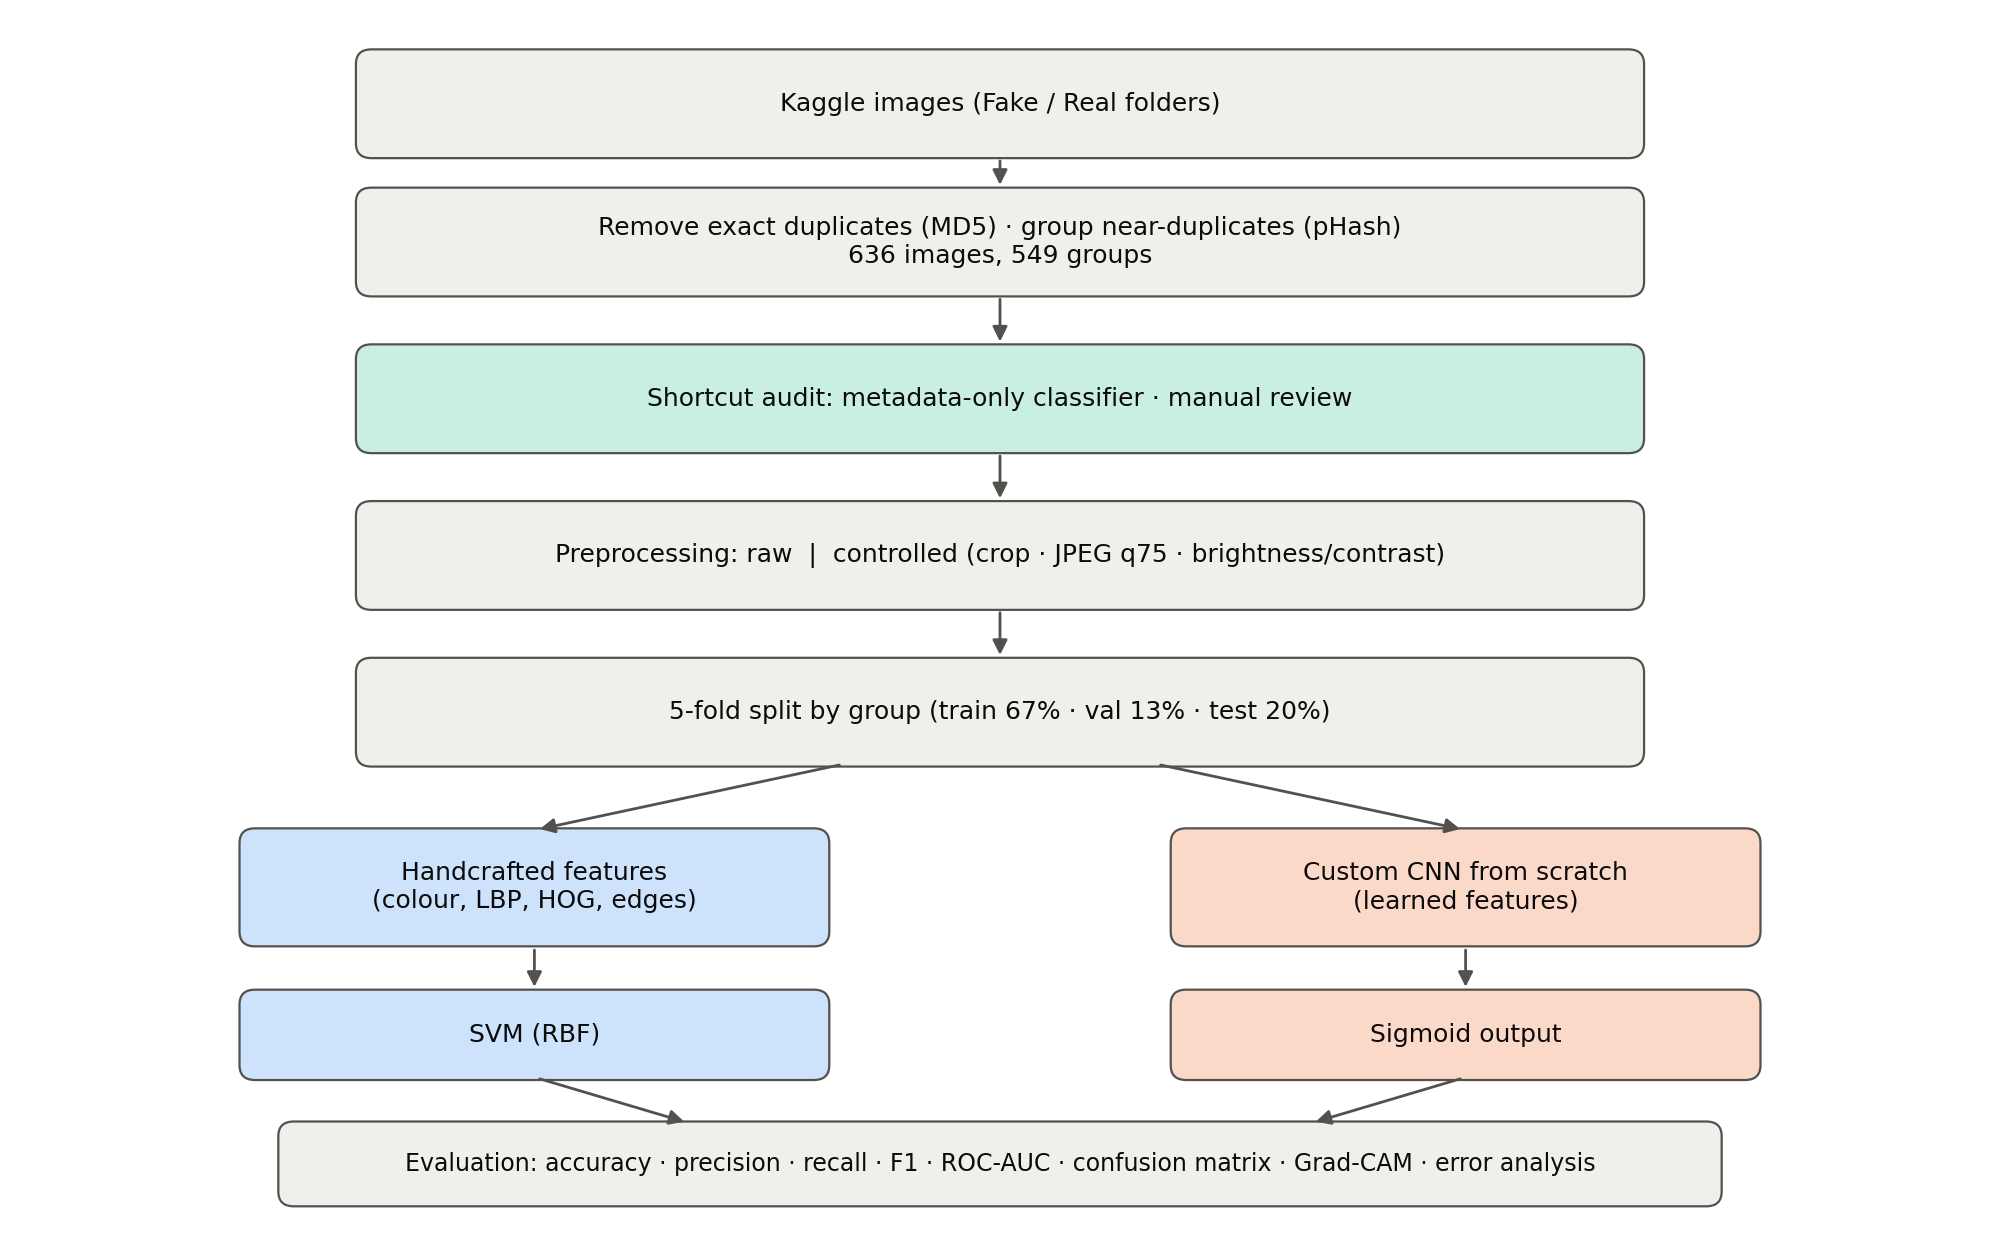
\includegraphics[width=0.92\columnwidth]{pipeline.png}
\caption{System pipeline. The audit (green) is run before any model is trained.}
\label{fig:pipeline}
\end{figure}

\begin{figure*}[t]
\centering
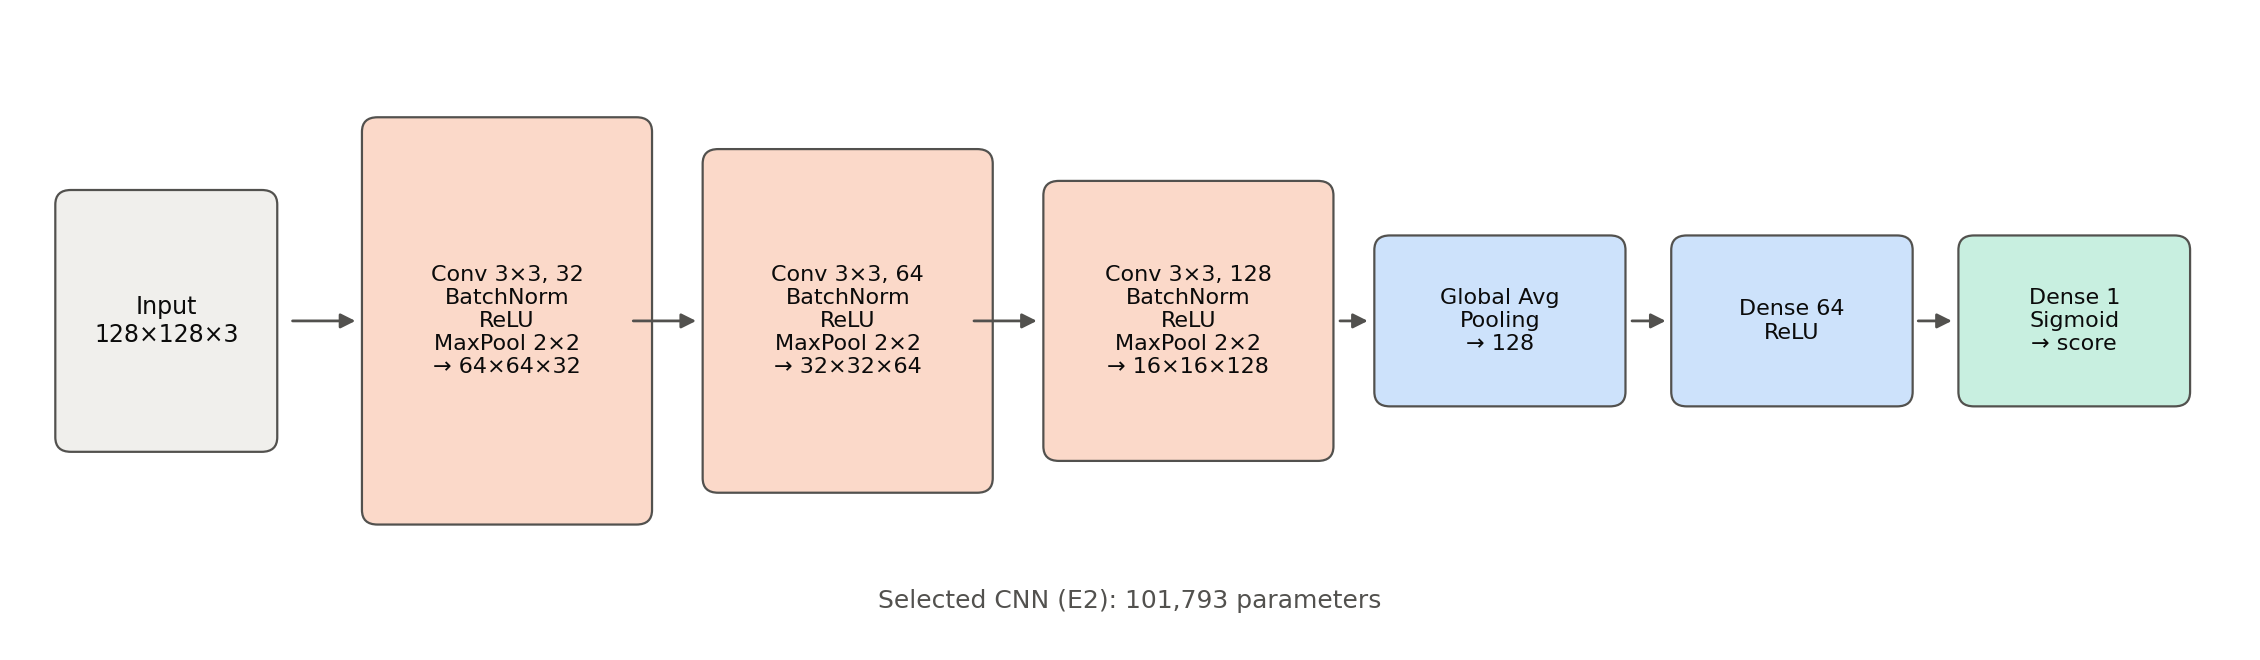
\includegraphics[width=0.9\textwidth]{cnn_architecture_selected.png}
\caption{Architecture of the selected CNN (E2), trained from scratch.}
\label{fig:arch}
\end{figure*}


\subsection{Provenance audit}
Before training any model, we wanted to know if the two classes differ in simple file details. For every image we recorded the file format, width, height, file size and average brightness. Then we trained a logistic-regression classifier on \emph{only these five numbers}, with the same grouped cross-validation. If this works well, it means the label can be guessed without even looking at the packaging. We also looked at 40 random images from each class by eye.

\begin{figure*}[t]
\centering
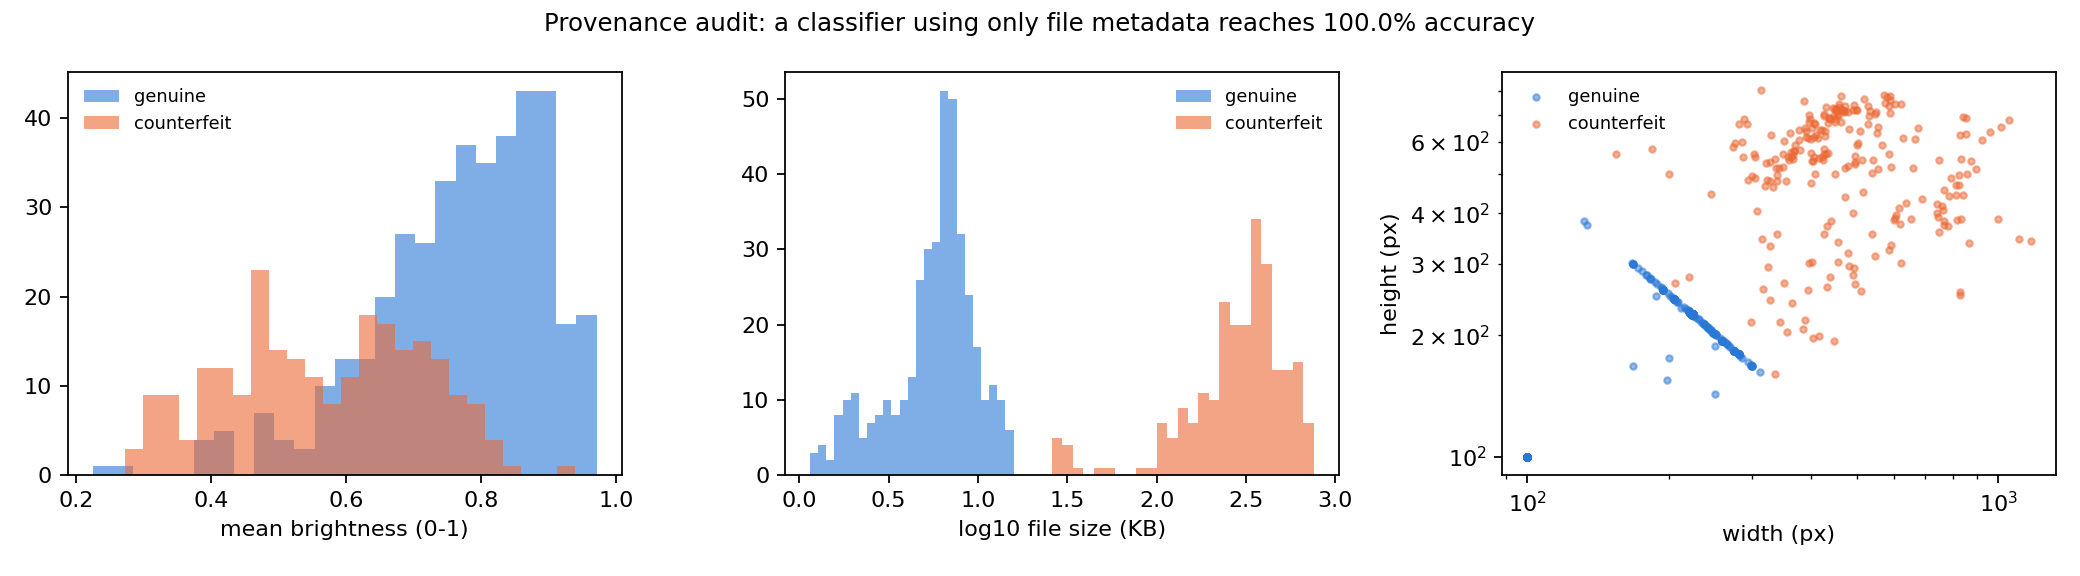
\includegraphics[width=0.95\textwidth]{audit_plots.png}
\caption{Provenance audit: brightness, file size and resolution by class. The classes are almost perfectly separated by properties unrelated to authenticity.}
\label{fig:audit}
\end{figure*}

\subsection{Preprocessing protocols}
Every image is converted to RGB (using its EXIF orientation) and made $128\times128\times3$. We tried two ways of doing this:
\begin{itemize}
\item \textbf{Raw:} just resize to $128\times128$, like a normal pipeline would.
\item \textbf{Controlled (ours):} resize the short side to 128 and crop the centre; save every image again as JPEG at quality 75, so both classes get the same compression; then fix the brightness and contrast in CIE-LAB space,
\begin{equation}
L' = \frac{L-\mu_L}{\sigma_L}\cdot 20 + 55,
\end{equation}
where $\mu_L$ and $\sigma_L$ are the mean and standard deviation of the image's lightness channel. The colours stay the same. This step does not use the labels at all, and we apply it in exactly the same way to every image, including the demo input.
\end{itemize}
We chose 128 as the input size because the genuine images are small (median $225\times225$ pixels, and 16\% are under 128 pixels on the short side). With a bigger input, most genuine images would be enlarged while the fake ones would be shrunk, which would add one more difference between the classes.

\subsection{Evaluation protocol}
We used stratified grouped 5-fold cross-validation (\texttt{StratifiedGroupKFold}). In each fold about 20\% of the groups go to the test set. The rest is split again into training (about 424 images) and validation (about 85 images, one sixth of the groups). We used the validation set only for early stopping and choosing the model, and the test set only for the final numbers. This way every image is tested exactly once, and we report the mean\,$\pm$\,standard deviation over the five folds. To see why grouping matters, we also made a normal random split. In that split, 138 test images (24--33 per fold) had a near-duplicate sitting in the training set. In the grouped split there were none, and a script checks this. We tested three settings: \emph{naive} (raw images, random split), \emph{leakage removed} (raw images, grouped split) and \emph{controlled} (controlled images, grouped split). The controlled setting is our main one.

\subsection{Baseline: handcrafted features and SVM}
For the baseline, each image is turned into 407 numbers: an HSV colour histogram (16 bins per channel, 48 values), RGB colour moments (6), uniform LBP histograms at two scales ($P{=}8,R{=}1$ and $P{=}16,R{=}2$; 28 values), HOG on a $64\times64$ greyscale image (9 orientations, $16\times16$ cells, $2\times2$ blocks; 324 values) and Canny edge density (1). We scale the features using the training set only and train an SVM with an RBF kernel and balanced class weights. In each fold we try $C\in\{0.1,1,10,100\}$ and $\gamma\in\{\text{scale},10^{-3},10^{-2}\}$ and keep the pair with the best validation F1.

\subsection{Proposed model: lightweight CNN trained from scratch}
Our network (Fig.~\ref{fig:arch}) has three convolution blocks. Each block is a $3\times3$ convolution with padding 1, then batch normalisation, ReLU and $2\times2$ max pooling. The blocks have 32, 64 and 128 filters. After that, global average pooling turns the $16\times16\times128$ feature map into a vector of 128 numbers, then comes a dense layer of 64 units with ReLU, and finally one output $z$. The counterfeit score is $s=\sigma(z)$. All weights start from PyTorch's normal random initialisation, and no pretrained weights are used anywhere. The whole model has 101{,}793 parameters.

\textbf{Training.} The data is imbalanced (62.6\% genuine), so we give more weight to the counterfeit class in the binary cross-entropy loss, using $w_+=N_{\text{gen}}/N_{\text{cf}}$ from the training set:
\begin{equation}
\mathcal{L} = -\frac{1}{N}\sum_{i=1}^{N}\Big[w_+\,y_i\log\sigma(z_i) + (1-y_i)\log\big(1-\sigma(z_i)\big)\Big].
\end{equation}
We train with Adam (learning rate $10^{-3}$), batch size 32 and at most 60 epochs. If the validation loss does not improve for 10 epochs we stop early and go back to the best weights. Each fold uses a fixed random seed so results can be repeated. When augmentation is on, we use random crops covering 85--100\% of the image, rotations up to $\pm10^\circ$ and $\pm10\%$ changes in brightness and contrast. We did not use flips, because real packaging never has mirrored text.

\textbf{Experiments.} We started from the network in our project proposal and changed one thing in each experiment (Table~\ref{tab:exp}). We picked the final model by the highest \emph{mean validation} ROC-AUC. The test folds were never used for this choice.

\begin{figure}[t]
\centering
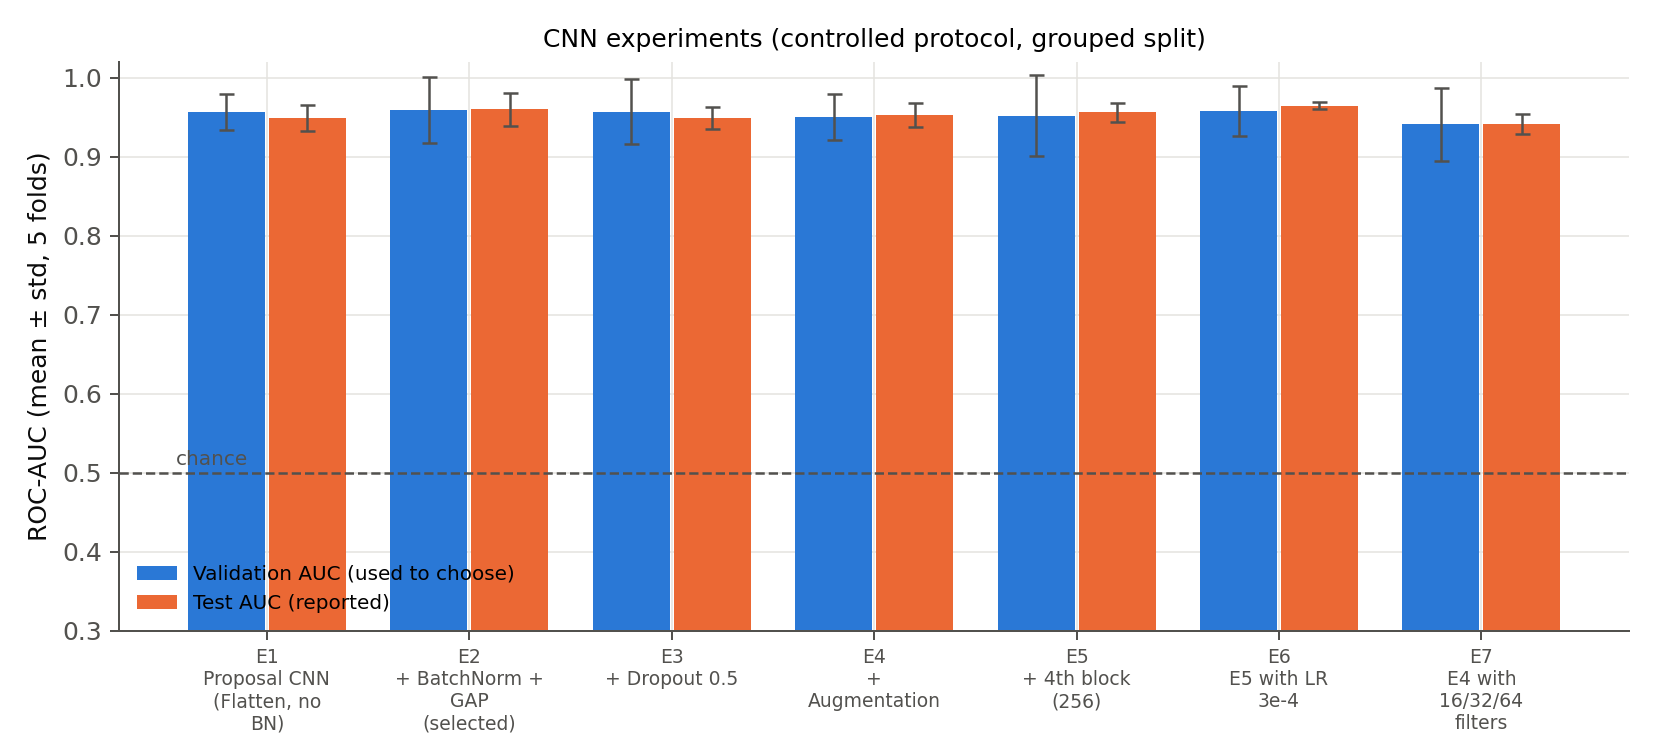
\includegraphics[width=\columnwidth]{cnn_experiments.png}
\caption{Validation AUC (used for selection) and test AUC of the seven CNN configurations.}
\label{fig:exp}
\end{figure}

\begin{figure}[t]
\centering
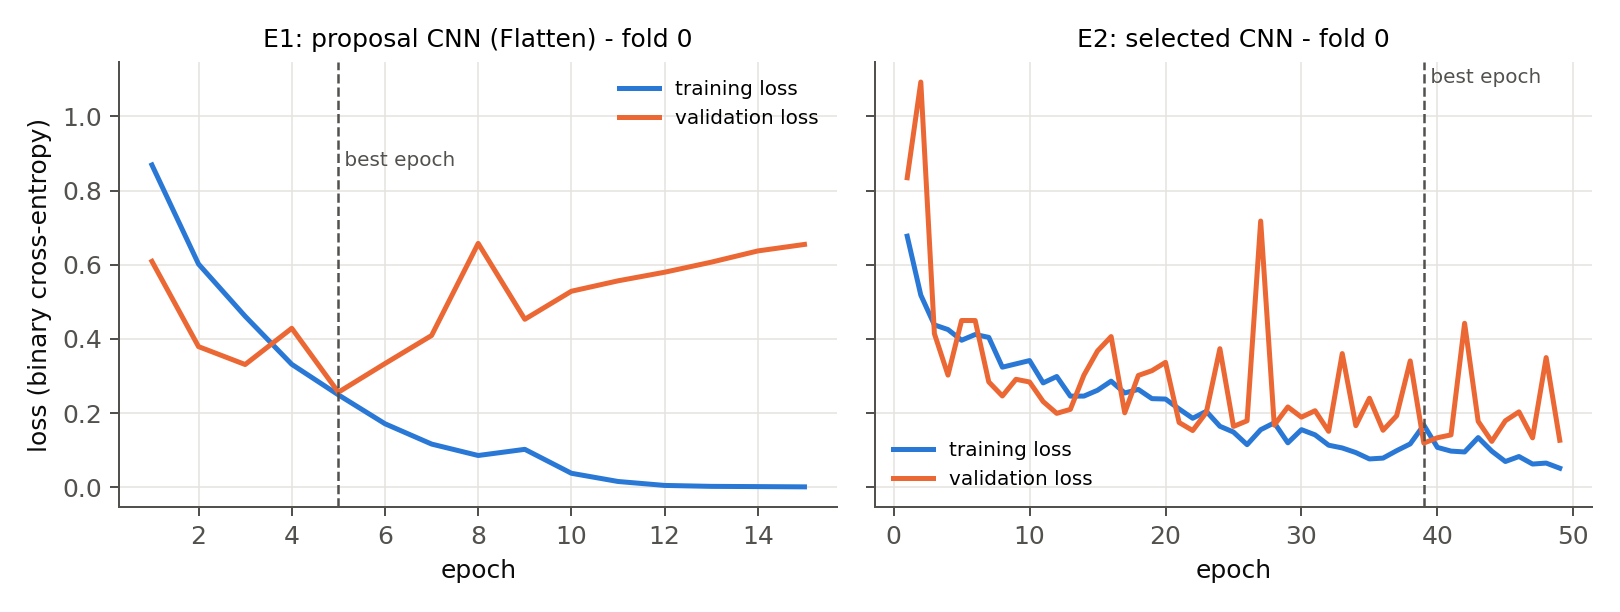
\includegraphics[width=\columnwidth]{training_curves.png}
\caption{Training and validation loss on fold 0: proposal CNN E1 (left) overfits after about five epochs; selected CNN E2 (right).}
\label{fig:curves}
\end{figure}

\subsection{Metrics and interpretation tools}
We treat counterfeit as the positive class. We report accuracy, balanced accuracy, precision $=\frac{TP}{TP+FP}$, recall $=\frac{TP}{TP+FN}$, $F_1=\frac{2PR}{P+R}$ and ROC-AUC. For us recall matters most, because missing a fake medicine is the worst mistake. We use a threshold of 0.5. To check if one model is really better than the other, we use an exact McNemar test on their predictions for the same images. To see where the CNN looks, we use Grad-CAM~\cite{selvaraju2017}, which weights the last convolution feature maps $A^k$ by their average gradients:
\begin{equation}
\alpha_k = \frac{1}{Z}\sum_{i,j}\frac{\partial z}{\partial A^k_{ij}}, \qquad
M = \mathrm{ReLU}\Big(\sum_k \alpha_k A^k\Big).
\end{equation}
Finally, we did a \textbf{background test}. We covered the middle $70\%\times70\%$ of every controlled image with flat grey, so only the outer 15\% border is left, and trained the SVM again on these images. If the border alone can predict the class, then the two classes differ in background or framing, not in the packaging.

%=====================================================================
\section{Results}
\begin{figure*}[t]
\centering
\begin{minipage}[b]{0.6\textwidth}\centering
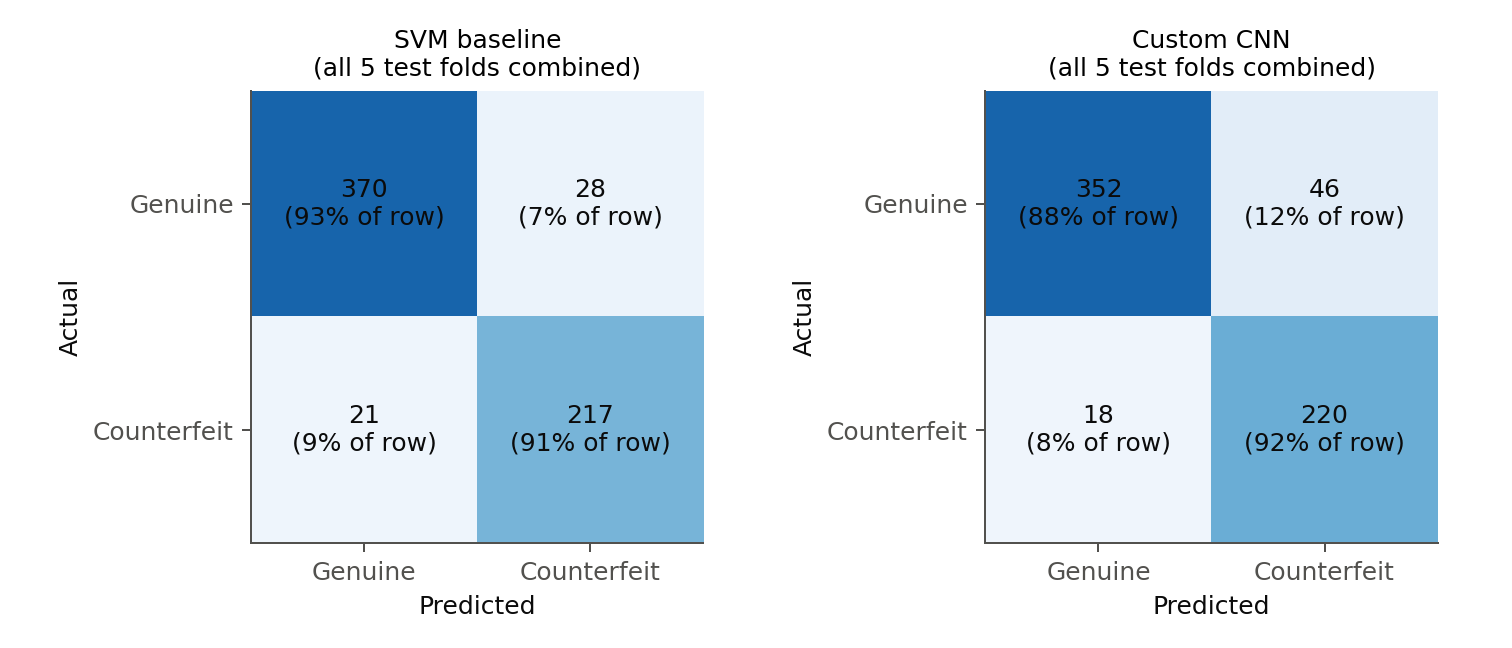
\includegraphics[width=\linewidth]{confusion_matrices.png}
\caption{Confusion matrices summed over the five test folds (636 predictions per model).}
\label{fig:cm}
\end{minipage}\hfill
\begin{minipage}[b]{0.36\textwidth}\centering
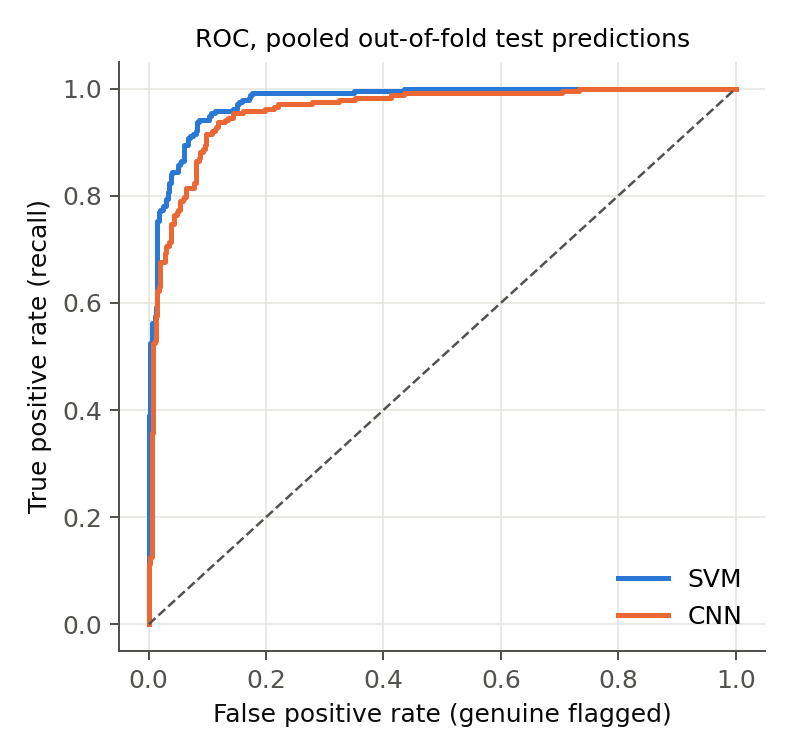
\includegraphics[width=\linewidth]{roc_curves.png}
\caption{ROC curves from pooled out-of-fold test predictions.}
\label{fig:roc}
\end{minipage}
\end{figure*}

\begin{figure}[!t]
\centering
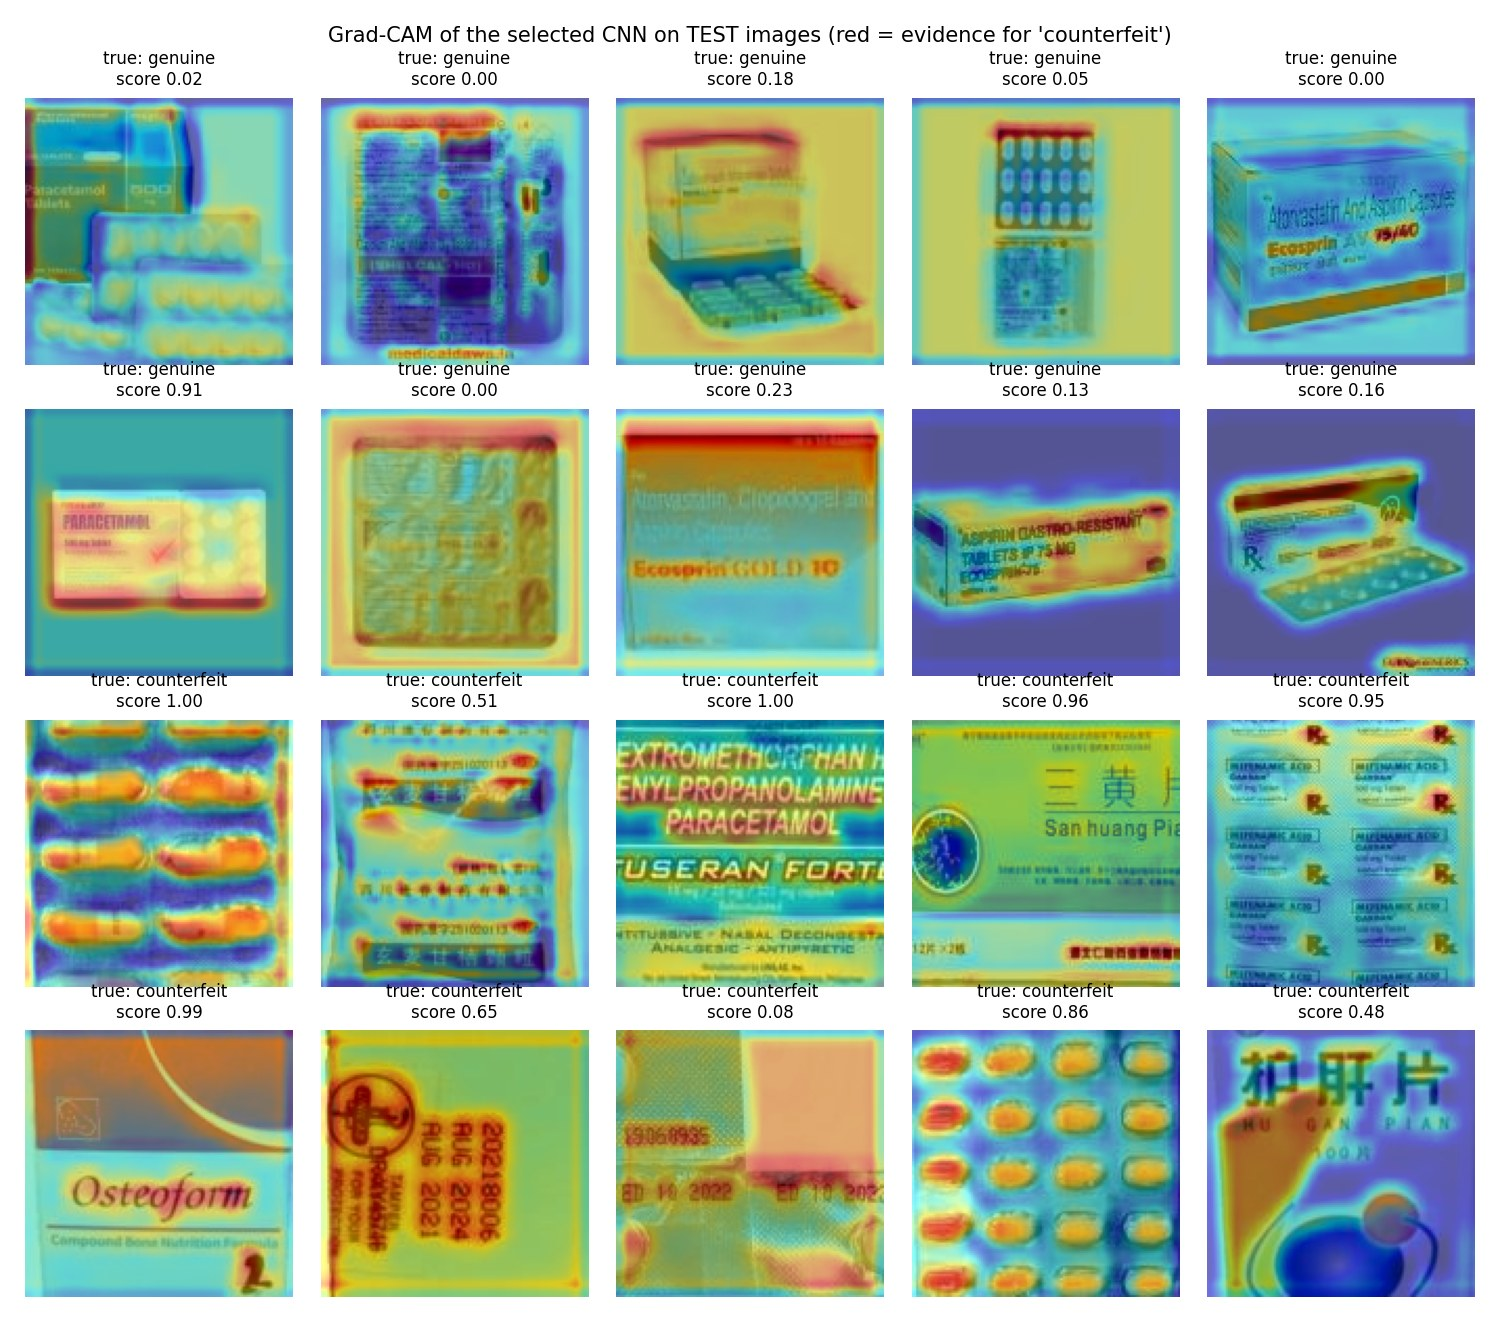
\includegraphics[width=0.92\columnwidth]{gradcam_examples.jpg}
\caption{Grad-CAM of the selected CNN on test images, each produced by the fold model that did not train on it (red = evidence for ``counterfeit'').}
\label{fig:gradcam}
\end{figure}


\subsection{Provenance audit}
Table~\ref{tab:audit} and Fig.~\ref{fig:audit} show that the two classes were clearly collected in different ways. Every genuine image is a small JPEG with a generic file name, and every counterfeit image is a large PNG screenshot. The classifier that only uses file details gets \textbf{100.0\%} accuracy. Even one simple rule, ``if it is a PNG, it is fake'', is 100\% correct. For comparison, always guessing the bigger class gives 62.6\%, and using brightness alone gives 75.2\%. Looking at the images by eye, we found content differences too: 26 of 40 genuine images have a plain light background, but only 3 of 40 fake ones do; 14 fake images have Chinese text and no genuine image does; and no brand appears in both samples. Most genuine images look like product photos from Indian online pharmacies, while most fake images are tight close-ups of blister packs and boxes.

\begin{table}[t]
\caption{Provenance audit: file properties by class}
\label{tab:audit}
\centering
\begin{tabular}{lcc}
\toprule
Property & Genuine & Counterfeit \\
\midrule
File format & JPEG (100\%) & PNG (100\%) \\
Median resolution (px) & $225\times225$ & $452\times549$ \\
Median file size & 6.4 KB & 324 KB \\
Mean brightness (0--1) & 0.77 & 0.57 \\
\midrule
Metadata-only classifier & \multicolumn{2}{c}{100.0\% accuracy} \\
\bottomrule
\end{tabular}
\end{table}

\subsection{CNN experiments}
Table~\ref{tab:exp} and Fig.~\ref{fig:exp} show the seven experiments. Our proposal network E1 has 4.29\,M parameters, and almost all of them are in the layer after flatten. Its validation loss is lowest at around epoch five and then goes up, while the training loss keeps going down to almost zero. This is clear overfitting (Fig.~\ref{fig:curves}). When we added batch normalisation and replaced flatten with global average pooling (E2), the model dropped to 101{,}793 parameters, \textbf{42$\times$ fewer}, and the mean test accuracy went up from 87.1\% to 89.9\%. E2 also had the highest mean validation AUC (95.9\%), so we selected it. Dropout, augmentation, a fourth block, a lower learning rate and fewer filters did not help more than the normal 2--5 point change between folds. E6 is basically tied with E2.

\begin{table*}[t]
\caption{CNN experiments (controlled protocol, grouped 5-fold CV; \%, mean $\pm$ std over folds). Selection uses validation AUC only.}
\label{tab:exp}
\centering
\begin{tabular}{llrcccccc}
\toprule
ID & Change from previous & Params & Best epoch & Val AUC & Test Acc & Test Recall & Test F1 & Test AUC \\
\midrule
E1 & Proposal CNN (Flatten, no BN) & 4{,}287{,}809 & 4.6 & \pmv{95.6}{2.2} & \pmv{87.1}{2.6} & \pmv{91.6}{3.0} & \pmv{84.3}{2.6} & \pmv{94.9}{1.6} \\
\textbf{E2} & \textbf{+ BatchNorm + GAP} & \textbf{101{,}793} & 20.6 & \textbf{\pmv{95.9}{4.2}} & \textbf{\pmv{89.9}{3.7}} & \textbf{\pmv{92.4}{3.9}} & \textbf{\pmv{87.4}{4.2}} & \textbf{\pmv{96.0}{2.1}} \\
E3 & + Dropout 0.5 & 101{,}793 & 20.6 & \pmv{95.7}{4.1} & \pmv{87.6}{3.0} & \pmv{87.4}{4.5} & \pmv{84.1}{3.5} & \pmv{94.9}{1.4} \\
E4 & + Data augmentation & 101{,}793 & 17.4 & \pmv{95.0}{2.9} & \pmv{89.2}{3.6} & \pmv{89.5}{4.0} & \pmv{86.2}{4.1} & \pmv{95.2}{1.5} \\
E5 & + 4th block (256 filters) & 405{,}409 & 18.6 & \pmv{95.2}{5.1} & \pmv{88.2}{3.5} & \pmv{89.5}{2.5} & \pmv{85.1}{3.8} & \pmv{95.6}{1.2} \\
E6 & E5 with learning rate $3\!\times\!10^{-4}$ & 405{,}409 & 22.2 & \pmv{95.8}{3.2} & \pmv{89.9}{2.3} & \pmv{92.0}{3.7} & \pmv{87.3}{2.5} & \pmv{96.5}{0.5} \\
E7 & E4 with 16/32/64 filters & 27{,}921 & 19.6 & \pmv{94.1}{4.6} & \pmv{87.4}{5.0} & \pmv{89.5}{9.9} & \pmv{84.1}{6.7} & \pmv{94.1}{1.3} \\
\bottomrule
\end{tabular}
\end{table*}

\subsection{CNN versus SVM}
Table~\ref{tab:main} compares our CNN with the SVM in the controlled setting, and Figs.~\ref{fig:cm} and~\ref{fig:roc} show the confusion matrices and ROC curves. The SVM is a little ahead on accuracy, F1 and AUC, but the ranges across folds overlap. Out of 636 images, 27 are wrong only for the SVM, 42 only for the CNN, and 22 for both. The McNemar test gives $p=0.09$, so the difference is \textbf{not significant} at the 5\% level. The two models also make different kinds of mistakes. The CNN misses fewer fakes (18 false negatives vs 21), but it wrongly flags more genuine images (46 false positives vs 28). With only about 424 training images per fold, this is what we expected: the SVM gets features that already describe colour, texture and edges, while the CNN has to learn all of this by itself from very little data. So for RQ1, our from-scratch CNN separates the two classes about as well as the handcrafted baseline, with the best recall and a very small model.

\begin{table}[t]
\caption{SVM vs CNN (controlled protocol, grouped split; \%, mean $\pm$ std over 5 test folds)}
\label{tab:main}
\centering
\setlength{\tabcolsep}{4pt}
\begin{tabular}{lcc}
\toprule
Metric & SVM (407 features) & CNN E2 (scratch) \\
\midrule
Accuracy & \pmv{92.3}{2.9} & \pmv{89.9}{3.7} \\
Balanced accuracy & \pmv{92.1}{2.9} & \pmv{90.4}{3.2} \\
Precision & \pmv{88.7}{5.2} & \pmv{83.2}{7.4} \\
Recall & \pmv{91.2}{3.4} & \pmv{92.4}{3.9} \\
F1 & \pmv{89.9}{3.8} & \pmv{87.4}{4.2} \\
ROC-AUC & \pmv{97.8}{0.8} & \pmv{96.0}{2.1} \\
\midrule
TN / FP / FN / TP & 370 / 28 / 21 / 217 & 352 / 46 / 18 / 220 \\
\bottomrule
\end{tabular}
\end{table}

\subsection{Shortcut study}
Table~\ref{tab:shortcut} answers RQ2. First, removing leakage and file-level differences did not change much. Across the three settings, SVM accuracy goes 93.7\%, 93.9\%, 92.3\%, and CNN accuracy goes 86.8\%, 89.0\%, 89.9\%, all within one or two standard deviations. This makes sense: resizing to $128\times128$ already hides the file format and size from the models, and there were not enough near-duplicates to change the average much. Second, and more important, the background test stays high. An SVM that never sees the packaging still gets \textbf{\pmv{90.7}{2.5}\%} accuracy (ROC-AUC \pmv{97.0}{1.0}\%), almost the same as the 92.3\% of the SVM that sees the whole image. So whatever separates the two classes is mostly in the background, framing and photo style, and our preprocessing cannot remove that.

\begin{table}[t]
\caption{Shortcut study: accuracy (\%) under each condition}
\label{tab:shortcut}
\centering
\setlength{\tabcolsep}{4pt}
\begin{tabular}{lcc}
\toprule
Condition & SVM & CNN \\
\midrule
Naive (raw, random split) & \pmv{93.7}{2.4} & \pmv{86.8}{3.9} \\
Leakage removed (raw, grouped) & \pmv{93.9}{1.3} & \pmv{89.0}{0.6} \\
Controlled (normalised, grouped) & \pmv{92.3}{2.9} & \pmv{89.9}{3.7} \\
\midrule
Background probe (border only) & \pmv{90.7}{2.5} & -- \\
Metadata only (5 file properties) & 100.0 & -- \\
Majority class & 62.6 & -- \\
\bottomrule
\end{tabular}
\end{table}

\subsection{Grad-CAM and error analysis}
On average, 46.5\% of the Grad-CAM heat for genuine test images and 49.1\% for fake ones is in the outer 15\% border, and that border is 51.0\% of the image area. So the CNN is not looking only at the border; its attention is spread over the whole image (Fig.~\ref{fig:gradcam}). For fake images, the heat is usually on pills, foil texture and printed text. For the catalogue-style genuine photos, it is often on the plain background or the edges of the box. Over all 636 test predictions, the CNN makes 64 mistakes (46 FP, 18 FN), and 21 of them are confident (score above 0.9 or below 0.1). The SVM makes 49 (28 FP, 21 FN). Most of the CNN's confident false positives are genuine images that look like the fake class in \emph{style}: close-ups of blister packs filling the frame, dark bands, and watermarked close-ups. Its false negatives include fake boxes with large plain light areas, which look like the genuine catalogue photos. Together with the background test, this tells us the two classes differ in overall photo style, and this shows up everywhere in the image.

%=====================================================================
\section{Discussion}
\textbf{RQ1.} A small CNN trained from scratch on about 424 images per fold gets 89.9\% accuracy and 92.4\% recall. Statistically, this is the same as a well-tuned handcrafted-feature SVM. The change that helped most was making the network more efficient: global average pooling with batch normalisation removed 97.6\% of the parameters, reduced overfitting and slightly improved accuracy. Adding regularisation or more layers did not make a clear difference with this little data.

\textbf{RQ2.} Our audit shows that these accuracies should not be taken as proof of detecting fakes. (i) File details alone predict the label perfectly, so the two classes were collected differently. (ii) The SVM that only sees the border gets 90.7\%, so the packaging is hardly needed at all. (iii) No brand is in both classes, so the product itself is mixed up with the label. (iv) The mistakes follow framing and style. Grouped splits and controlled preprocessing are still needed, but here they changed the numbers only a little, which shows that the remaining signal is inside the image content. Since no product appears in both classes, this dataset cannot tell us how much of the accuracy, if any, comes from real signs of a fake.

\textbf{Comparison with the base paper.} Ramos \emph{et al.}~\cite{ramos2024} report about 88.75\% on their own photos of one product taken with one camera. Our numbers come from a different, web-collected dataset with a different test setup, so the two cannot be compared directly, and we do not claim to beat them. In fact, our audit supports their approach of taking both classes with the same camera setup. Without checking how the data was collected, accuracy alone cannot tell a fake detector apart from a model that just recognises where the photo came from.

\textbf{Limitations.} The dataset is small (636 images, about 127 per test fold), we cannot check if its labels are correct, and we had no separate external test set. Perceptual hashing with a fixed threshold can miss copies that were edited a lot. The model's scores are not calibrated probabilities. And checking the packaging photo can never fully prove whether a medicine is real.

%=====================================================================
\section{Conclusion and Future Work}
In this project we built a complete pipeline for checking packaging images that anyone can run again: duplicate removal, grouped cross-validation, a handcrafted-feature SVM, a 101{,}793-parameter CNN trained from scratch and chosen through seven experiments, Grad-CAM, error analysis and a web demo. Our CNN gets 89.9\% accuracy, 96.0\% ROC-AUC and 92.4\% recall on fakes. This matches the SVM within statistical noise, and the CNN is 42$\times$ smaller than our first design. Our shortcut audit shows that on this public dataset, file details alone give 100\% accuracy and the image border alone gives 90.7\%, so high accuracy here does not prove that a model can detect fakes. These audit tests are easy to run, and we think they should be a standard check before anyone reports results in this area.

In the future, we would like to: (1) collect proper matched data, with the same products photographed as genuine and fake using the same camera, lighting and background, for example together with a drug regulator or a pharmacy lab; (2) only trust results when the file-details and border tests are close to chance; (3) test on a separately collected test set; (4) add text checks with OCR (spelling, batch numbers, dates) and look at security features; (5) detect and crop the package first, so the background is removed before classification; and (6) calibrate the scores so the model can be used in a mobile app.

\section*{Code Availability}
All our code, the trained model, the results for every fold and the demo are available at \url{\repourl}.

\section*{Acknowledgment}
The authors thank the Department of Information Technology, Netaji Subhas University of Technology, New Delhi, for supporting this work.

\balance
\begin{thebibliography}{00}
\bibitem{ramos2024} R. R. T. Ramos, K. R. B. Samonte, and C. O. Manlises, ``Medicine authentication based on image processing using convolutional neural networks,'' in \textit{Proc. 16th Int. Conf. Computer and Automation Engineering (ICCAE)}, IEEE, 2024, pp. 278--282, doi: 10.1109/ICCAE59995.2024.10569752.
\bibitem{zakaria2025} Y. Zakaria, E. Ishidera, R. Ishiyama, T. Matsui, H. Suwa, Y. Matsuda, and K. Yasumoto, ``Counterfeit medicine detection by visual inspection of package design using multimodal LLMs with text and image prompt engineering,'' in \textit{Proc. Int. Conf. Intelligent Medicine and Image Processing (IMIP 2025)}, Proc. SPIE, vol. 13658, 2025, pp. 92--99, doi: 10.1117/12.3071640.
\bibitem{kaggle} surajkumarjha1, ``Fake vs real medicine datasets images,'' Kaggle. [Online]. Available: https://www.kaggle.com/datasets/surajkumarjha1/fake-vs-real-medicine-datasets-images
\bibitem{provenance2026} sophiezla, ``Provenance confounding in image authenticity classification,'' code and manuscript, GitHub/Zenodo, 2026, doi: 10.5281/zenodo.21936720.
\bibitem{geirhos2020} R. Geirhos, J.-H. Jacobsen, C. Michaelis, R. Zemel, W. Brendel, M. Bethge, and F. A. Wichmann, ``Shortcut learning in deep neural networks,'' \textit{Nature Machine Intelligence}, vol. 2, pp. 665--673, 2020.
\bibitem{zech2018} J. R. Zech, M. A. Badgeley, M. Liu, A. B. Costa, J. J. Titano, and E. K. Oermann, ``Variable generalization performance of a deep learning model to detect pneumonia in chest radiographs: A cross-sectional study,'' \textit{PLOS Medicine}, vol. 15, no. 11, e1002683, 2018.
\bibitem{cortes1995} C. Cortes and V. Vapnik, ``Support-vector networks,'' \textit{Machine Learning}, vol. 20, pp. 273--297, 1995.
\bibitem{dalal2005} N. Dalal and B. Triggs, ``Histograms of oriented gradients for human detection,'' in \textit{Proc. IEEE CVPR}, 2005, pp. 886--893.
\bibitem{ojala2002} T. Ojala, M. Pietik\"ainen, and T. M\"aenp\"a\"a, ``Multiresolution gray-scale and rotation invariant texture classification with local binary patterns,'' \textit{IEEE Trans. Pattern Anal. Mach. Intell.}, vol. 24, no. 7, pp. 971--987, 2002.
\bibitem{ioffe2015} S. Ioffe and C. Szegedy, ``Batch normalization: Accelerating deep network training by reducing internal covariate shift,'' in \textit{Proc. ICML}, 2015, pp. 448--456.
\bibitem{srivastava2014} N. Srivastava, G. Hinton, A. Krizhevsky, I. Sutskever, and R. Salakhutdinov, ``Dropout: A simple way to prevent neural networks from overfitting,'' \textit{J. Mach. Learn. Res.}, vol. 15, pp. 1929--1958, 2014.
\bibitem{lin2014} M. Lin, Q. Chen, and S. Yan, ``Network in network,'' in \textit{Proc. ICLR}, 2014.
\bibitem{kingma2015} D. P. Kingma and J. Ba, ``Adam: A method for stochastic optimization,'' in \textit{Proc. ICLR}, 2015.
\bibitem{selvaraju2017} R. R. Selvaraju, M. Cogswell, A. Das, R. Vedantam, D. Parikh, and D. Batra, ``Grad-CAM: Visual explanations from deep networks via gradient-based localization,'' in \textit{Proc. IEEE ICCV}, 2017, pp. 618--626.
\end{thebibliography}

\end{document}
